
\section{Introduction}
AHIR provides a platform to translate an algorithm described in a high level programming language like C to a VHDL circuit description. In this work, we characterise the resulting hardware in terms of physical and performance parameters such as area, power and delay. Our approach followed for obtaining layout from a VHDL description is as shown in the Fig. 1.


\begin{figure}[ht]
{\centering \resizebox*{6in}{4in}{\includegraphics{list_of_figures1.ps}} \par}
\caption{Flow describing VHDL Description to Layout}
\end{figure}

At each level, a different tool is used for a specific purpose. At first,  the VHDL code is simulated and checked for  its functionality using ModelSim 6.3a. The next step is  to perform synthesis and obtain a gate level netlist. For all our circuit examples we have used the OSU Standard Cell library for TSMC 0.18 technology and Synopsis  Design Compiler (DC) to perform synthesis. The netlist thus obtained is used as an input to Cadence SOC Encounter to generate the layout. 

The memory is designed as single bank or as a combination of multiple banks. The later would aid parallelism in the circuit. Also, the memory could be pipelined. We have explored 6 different memory architectures for different examples and compared the performance of the circuits with multiple banks versus single banks, pipelined as opposed to non-pipelined memory. 
